\chapter{Appendix}
\begin{figure}[!h]
	\centering
	\subfloat{
		\subfigimg[height=150pt]{a}{Ressources/Differential/Bottom}	
	} \hfill
	\subfloat{
		\subfigimg[height=150pt]{b}{Ressources/Differential/Top}	
	}
	\capption{Flow Rate Dependency of Differential Counting Setup}{(\textbf{a}) Optimized for top sensor (\textbf{b}) Optimized for bottom sensor}
	\label{fig:diff:flowRate}
\end{figure}

\begin{figure}[!h]
	\centering
	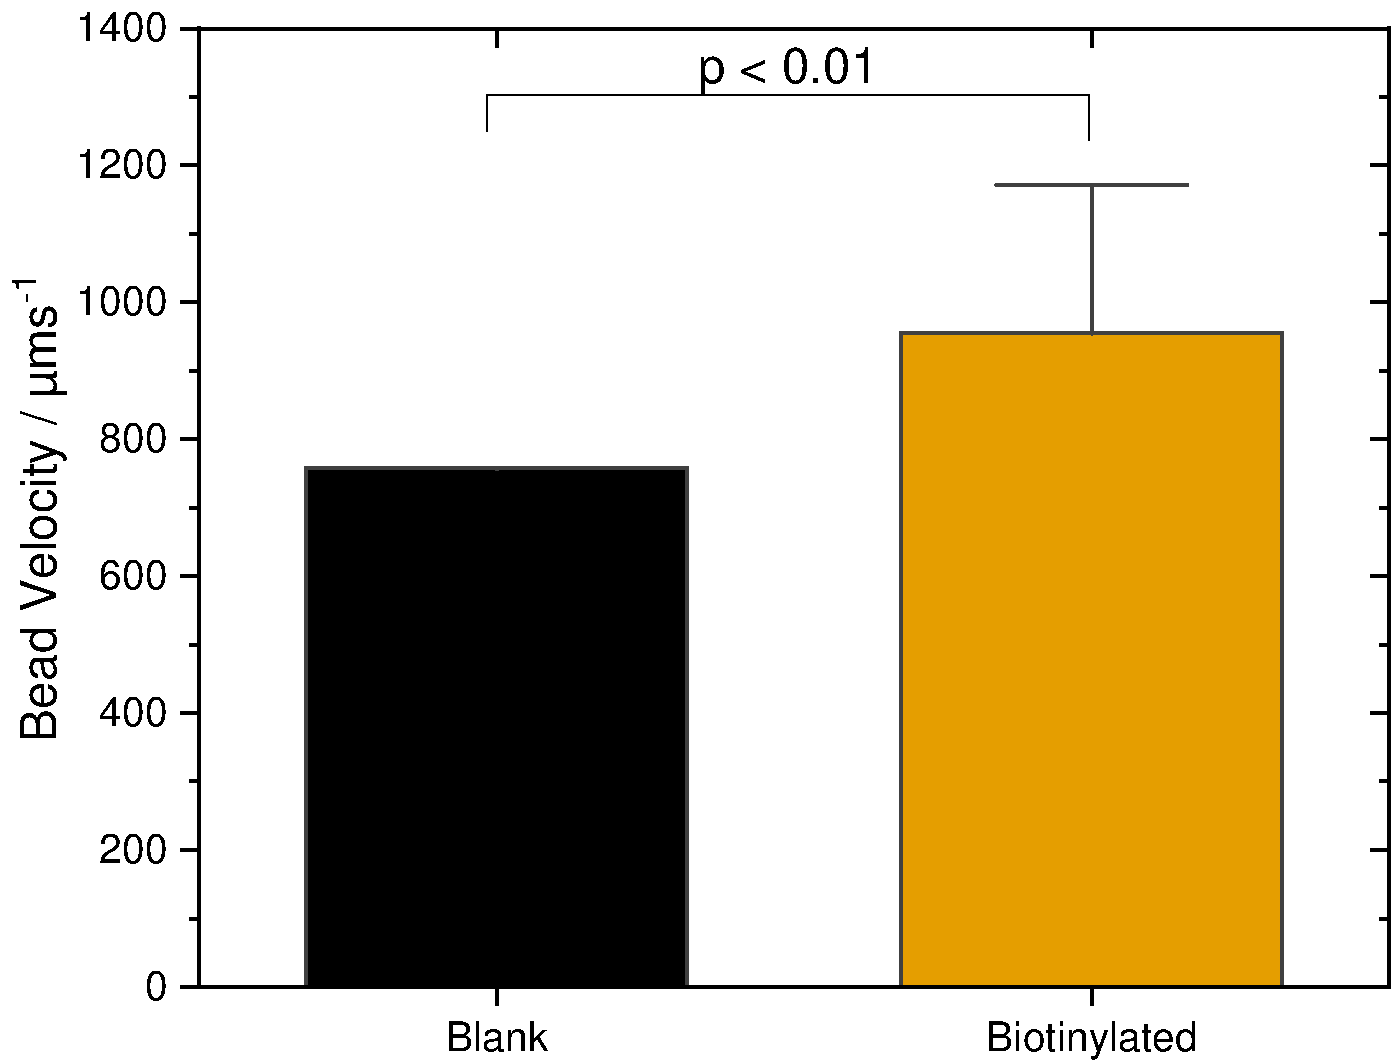
\includegraphics[width=.3\linewidth]{Ressources/Concentration/CaptureVelocity}
	\capption{Measured Bead Velocity}{ Not sure what to say about velocity itself. Maybe remove completely,   p < 0.01}
	\label{fig:conc:vel}
\end{figure}

\begin{figure}
	\centering
	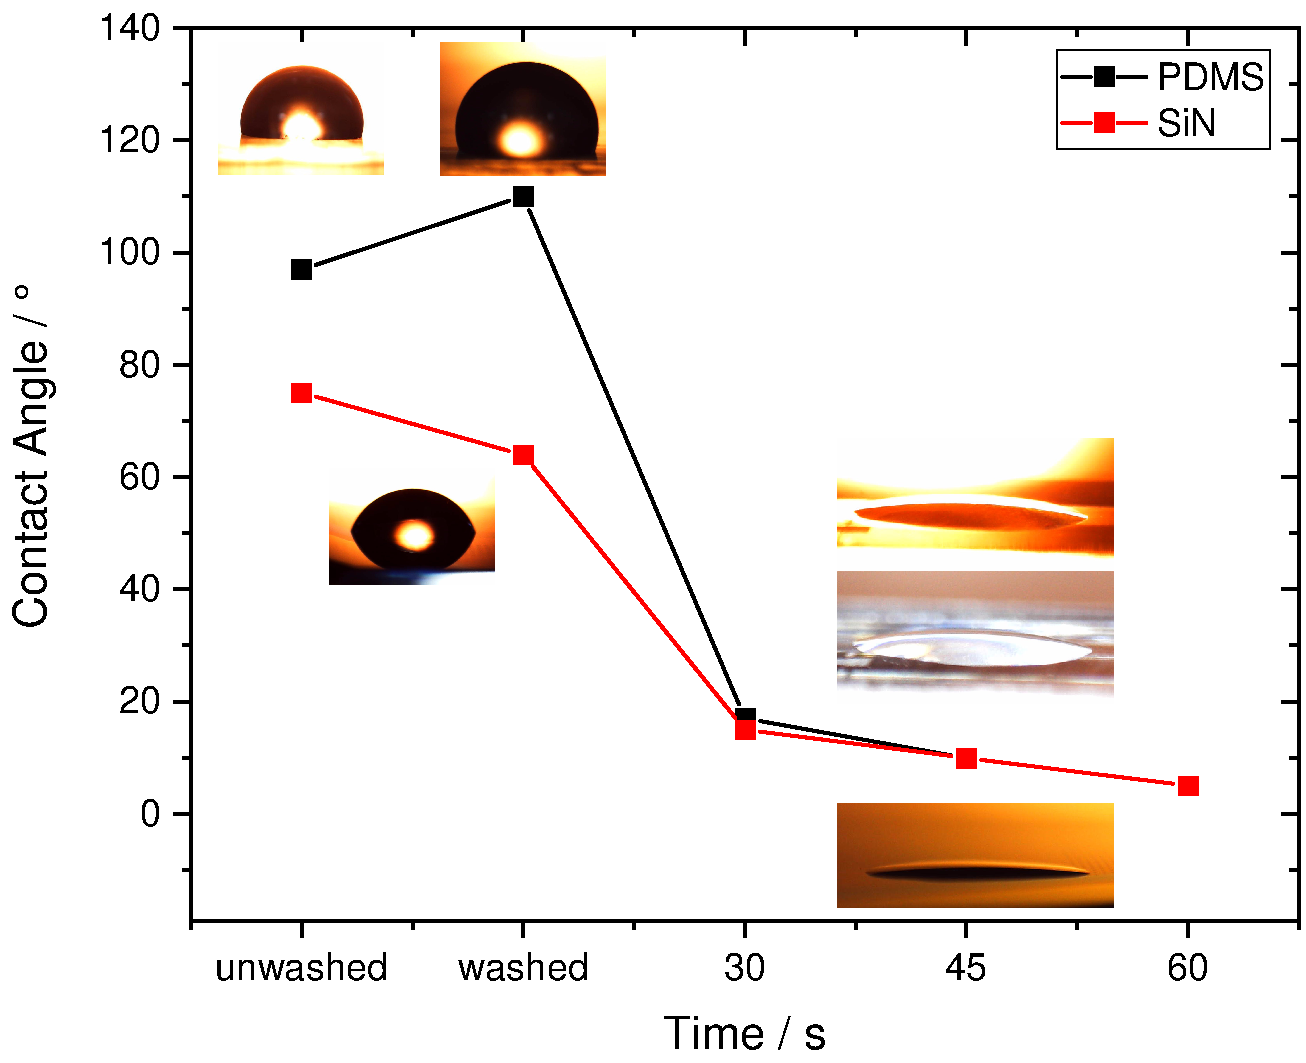
\includegraphics[height=150pt]{Ressources/ResultPlots/PDMS-sessileDrop}
	\capption{Hydrophobicity Analysis of \gls{pdms} under Plasma Exposure}{For an optimal plasma bond to glass, \gls{sin} and \gls{pdms}, the contact angle was measured after treatment. The initial decrease until \SI{45}{\second} declares the optimum around this time. Longer times should be avoided consequently to prohibit further surface damages by reactive ions. }
	\label{fig:coval:plasma}
\end{figure}

